\section{Continuum Mechanics}

\subsection{Course Overview}
This course is a topics course in many-body dynamics. What does that mean? It is inspired by a Polykov used to teach in Princeton, called ``Topics'', where he would arrive 10 minutes before and decide what would be an important topic in theoretical physics to teach. I (Vincenzo) don't have quite this level of improvisation, but this will largely be a course in research topics of non-equilibrium many-body physics/active matter.

We do have a broad theme - we want to treat various aspects of physics (mechanics, solid physics, phase transitions) from the perspective of dynamical systems. The formal pre-reqs are the intro soft matter course (currently being taught in parallel) as well as a course in statical field theory, but these are in some sense excessive - an enterprising student would be able to follow along, with some additional reading.

There is a recommended book (Soft Matter by Vitelli and others). The book will make the lectures look good in that the lectures will have better explanations. But since this course is being taught for the first time, there will be no lecture notes, so some sections of the book may be useful.

Assessment will be from problem sets (3 problem sets of 3-4 problems each). They may be difficult (they will be taken from the book) and long, but they will be stimulating and well written out. They will largely be mini research topics (it will be like working on research with a soft matter theorist like me (Vincenzo), or perhaps someone less crazy) - the grading will be lenient accordingly, as well as policies around deadlines, working together.

\subsection{Continuum Mechanics Review}

We will start by looking at equilibrium theory of physics, by looking at elasticity. This is normally a problem treated in the context of variational classical field theory. But we will approach this problem from a non-variational perspective (odd elasticity), and we will see interesting phenomena - namely chaos - emerge.

Our starting point is Newton's second law:
\begin{equation}
    \v{F} = \dod{\v{p}}{t}
\end{equation}

For continuous media, we can consider the force as coming from a volume integral of the pressure over space:
\begin{equation}
    f_i = \dod{}{t}\iiint dV P_i = \oiint dA \sigma_{ij}n_j
\end{equation}
where we have used Stoke's theorem to rewrite the volume integral as an integral over the area. 

\begin{center}
    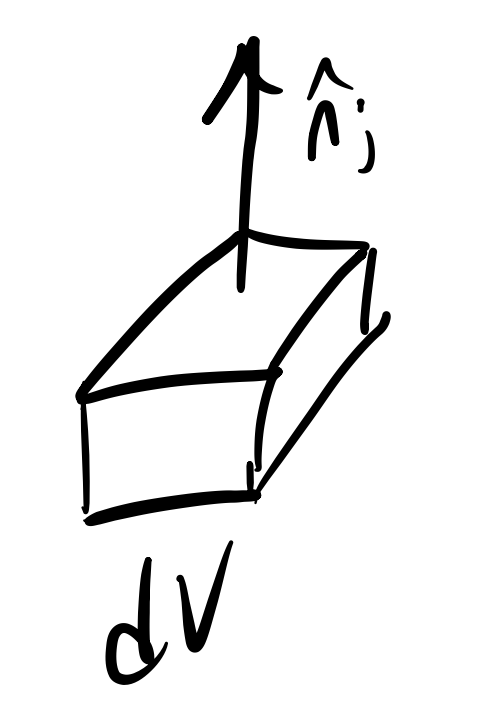
\includegraphics[scale=0.35]{Lectures/Images/lec1-volelement.png}
\end{center}

Therein, $\sigma_{ij}$ is the linear momentum flux, or a rank-2 stress tensor. Note that throughout, we use Einstein summation convention where repeated indices are summed over (e.g. $u_{ij}x_j \coloneqq \sum_j u_{ij}x_j$).

We can further write:
\begin{equation}
    f_i = \iiint \dpd{\sigma_{ij}}{x_j}dV
\end{equation}
Another way to package this; we can write the force as a volume integral of a force density, which is a divergence of the stress tensor:
\begin{equation}
    f_i = \iiint dV F_i
\end{equation}
with:
\begin{equation}\label{eq:forcedensity}
    \boxed{F_i = \p_j \sigma_{ij}}
\end{equation}
one can also take this as the definition of the stress tensor. If you have never seen the stress-tensor, it is recommended you read the first chapter of Soft Matter.

There is an assumption we made here. When we set the volume integral of $dVP_i$ equal to the area integral, we assumed that there were no sources. We will see what happens soon when this assumption is violated. For example we may have a solid immersed in a fluid, in which case Newton's third law may not hold and linear momentum is generically not conserved. One thing that this class will emphasize is what happens to the conclusions when assumptions are challenged!

Let's look at a differential of the force density:
\begin{equation}
    dF_i = \sigma_{ij}n_j dA
\end{equation}
As a concrete example, we can look at the forces acting on different faces of our cube:

\begin{center}
    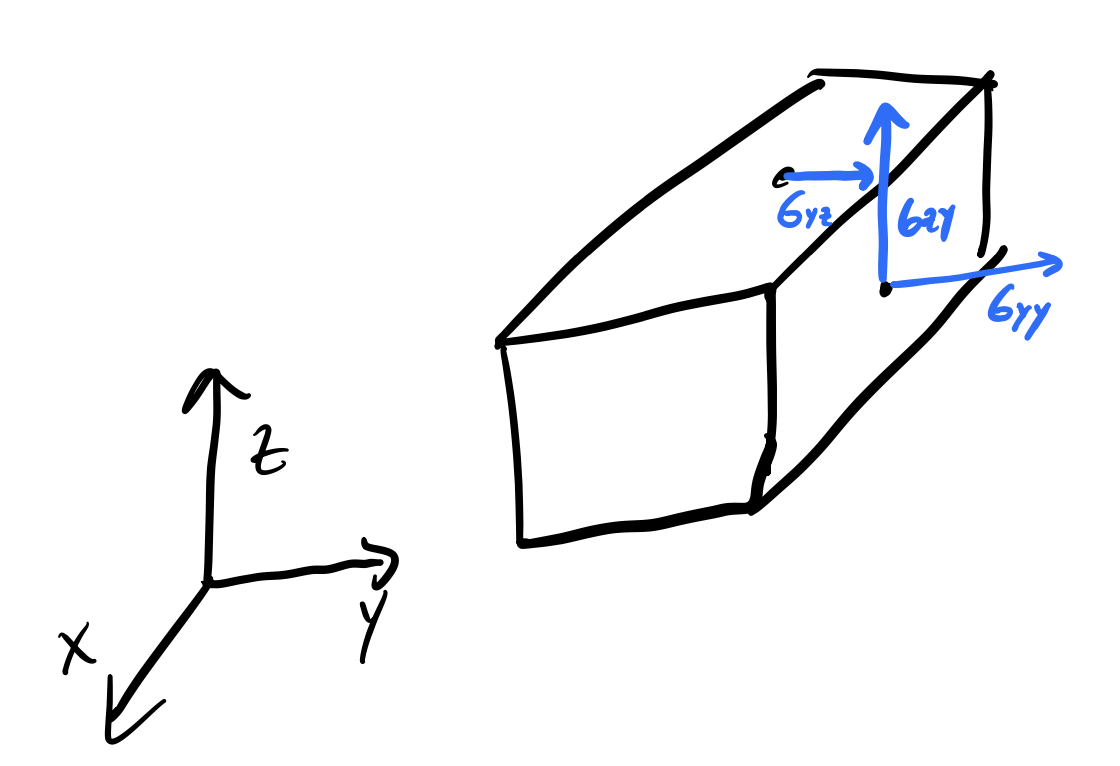
\includegraphics[scale=0.35]{Lectures/Images/lec1-forces.png}
\end{center}

\subsection{Constitutive Equation and Conservation Laws}
We want a relationship between the stress tensor and the order parameter, relating to the displacements. We assume that there is translation invariance for now, so there is no dependence on the displacements themselves, only on gradients of the displacements (this is not true always, e.g. in the case of a solid in fluid, or a solid on a table with glue - these will be additional terms that we consider later). In linear response theory, we connect the stress and strain tensors (rank-2) via a stiffness tensor (rank-4):
\begin{equation}
    \sigma_{ij} = K_{ijkl}\p_k u_l = K_{ijkl}u_{kl}
\end{equation}
The above is a linearized constitutive equation. As ugly as the $K_{ijkl}$ above may be, forms the identity of the material. This is ``Hooke's Law on steroids''. Note that if we assume that microscopically a solid is composed of masses connected by Hookian springs with spring constant $k$, it is possible to derive the macroscopic stiffness tensor from the microscopic theory; this may be one of your problems later.

In 2-D, we have:
\begin{equation}
    u_{kl} = \m{\p_x u_x & \p_x u_y \\ \p_y u_x & \p_y u_y}
\end{equation}
\begin{equation}
    \sigma_{ij} = \m{\sigma_{xx} & \sigma_{xy} \\ \sigma_{yx} & \sigma_{yy}}
\end{equation}
Note that we do not symmetrize here. In fact we can explicitly think about what happens in the cases when the off-diagonal entries are not equal. When $\sigma_{ij} \neq \sigma_{ji}$, it means that there is a non-vanishing net-torque (imagine back to the forces on the cube picture) and so the medium can spontaneously rotate. What does this teach us? Buried in the cumbersome algebraic structure of the rank-4 tensor, we see the presence and or violation of conservation laws. In this case, $\sigma_{ij} \neq \sigma_{ji}$ it implies that angular momentum is \emph{not} conserved. Most books assume the fundamental conservation laws of nature hold and write down theories accordingly. But, we can allow for exotic mechanisms of the breaking of such fundamental laws, e.g. from interactions with external sources which give rise to effective theories.

We are rapidly marching through conservation laws; we have imposed conservation of linear momentum from the get-go, but we do not impose $\sigma_{ij} = \sigma_{ji}$/impose angular momentum conservation (If we did, then the rank-4 tensor would reduce to rank-3). This means that we have external torques present/sources of angular momentum. As we go on, we will study symmetries of our system through the symmetries of the (admittedly complicated) $K_{ijkl}$ object, and understand the conservation laws through it.

Now, we \emph{assume} that there is a potential energy. In Hooke's law, we assume $F = -\p_x E$ with $E = \frac{1}{2}kx^2$ so we have a conservative force. Here, we don't work on the level of single particles, so we write the total potential energy as the integral over energy density:
\begin{equation}
    U = \iiint d^3x \e(\v{x})
\end{equation}
The question is now what is $\e(\v{x})$? If we want a linear force, we require that $\e(\v{x})$ be a quadratic form in $\v{x}$:
\begin{equation}
    \e(\v{x}) = \frac{1}{2}c_{ijkl} u_{ij}(\v{x})u_{kl}(\v{x})
\end{equation}
Now, we want the force in the $l$th direction, which is a functional derivative of the energy density:
\begin{equation}
    \left(\text{Force}\right)_l = -\frac{\delta \e}{\delta u_l} = -\left(\dpd{\e}{u_l} - \p_k \dpd{\e}{u_{lk}}\right)
\end{equation}
where again we recall $u_{lk} = \p_l u_k$. Let's try to unweird this expression via analogy (maybe you want to explain to a friend, or pick up someone at a bar by telling them that you work on functional derivatives) - in classical mechanics, we have an action:
\begin{equation}
    S = \int L(q(t))dt
\end{equation}
we then have the trajectory that is followed is that for which the functional derivative of the action vanishes\footnote{Of course, this is something your date is expected to know.}:
\begin{equation}
    \frac{\delta S}{\delta q} = 0 \implies \dpd{L}{q_j} - \dod{}{t}\left(\dpd{L}{\dot{q}_i}\right) = 0
\end{equation}
And we can now see that the form of this expression is equivalent to the functional derivative of the energy density we wrote above.

Since we that the energy density cannot depend on displacement $u_l$/it only depend on gradients of displacement; hence the first term of the force expression vanishes:
\begin{equation}
    \left(\text{Force}\right)_l = \p_k \dpd{\e}{u_{lk}}
\end{equation}
Now if we recall Eq. \eqref{eq:forcedensity} that the force density is the divergence of the stress tensor, we can write the above as:
\begin{equation}
    \sigma_{lk} = \dpd{\e}{u_{lk}}
\end{equation}
Now, if $\e$ is quadratic in $u$, we will find that the relationship of stress and strain will be linear. The question then becomes; what is the relationship between $K_{ijkl}$ and between $c_{ijnm}$ (the coefficients of force and the coefficients of energy)? In the Hooke's law case they coincide and are both the spring constant $k$. However, this coincidence is only because we have a conservative force - we will see that even in this more general/continuum setting that if we have energy conservation the coefficients coincide, and in non-conservative settings they may differ.

Let us work through the algebra. Computing the derivative of $\e$:
\begin{equation}
    \begin{split}
        \dpd{\e}{u_{pq}} &= \frac{1}{2}c_{ijkl}\left[\delta_{ip}\delta_{jq}u_{kl} + u_{ij}\delta_{pk}\delta_{ql}\right] 
        \\ &= \frac{1}{2}\left[c_{pqkl}u_{kl} + c_{ijpq}u_{ij}\right]
        \\ &= \frac{1}{2}\left[c_{pqkl}u_{kl} + c_{klpq}\right]u_{kl}
    \end{split}
\end{equation}
Note in the third equality we replace $ij$ with $kl$; they are dummy/repeated/summed over indices and thus we can call them whatever we want\footnote{Name-calling is not good, but its ok with tensors - they don't mind.}. Now, identifying:
\begin{equation}
    K_{pqkl} = \frac{1}{2}[c_{pqkl} + c_{klpq}]
\end{equation}
we have:
\begin{equation}
    \sigma_{pq} = K_{pqkl}u_{kl}
\end{equation}
And thus we manifestly see that the stiffness tensor is symmetric under interchange of pairs of indices, so long as the force is derived from a variation of a quadratic energy density:
\begin{equation}
    \boxed{K_{pqkl} = K_{klpq}}
\end{equation}
This relation is known as the Maxwell-Betti reciprocity. Later we will identify $\alpha \coloneqq pq$ and $\beta \coloneqq kl$ and better appreciate the symmetry algebraically.

\subsection{Non-Conservative Forces}
What if we have a world where we deform the material and through interaction with the environment, the system can suck up or expel energy? Then, we will find that work is not a state function, and:
\begin{equation}
    \oint \v{F} \cdot d\v{l}\neq 0 
\end{equation}
In this context, the linear stress-strain relation says \emph{nothing} about the conservative nature of the forces, only that the forces are linear. It only says something about the energy with the constraint that the forces are conservative.

How do we think about the tensors in this setting? Recall that we can always write a tensor in terms of a symmetric and antisymmetric part, e.g.:
\begin{equation}
    \sigma_{ij} = \sigma_{ij}^S + \sigma_{ij}^A
\end{equation}
with:
\begin{equation}
    \sigma_{ij}^S = \frac{\sigma_{ij} + \sigma_{ji}}{2}, \quad \sigma_{ij}^S = \sigma_{ji}^S
\end{equation}
\begin{equation}
    \sigma_{ij}^A = \frac{\sigma_{ij} - \sigma_{ji}}{2}, \quad \sigma_{ij}^A = -\sigma_{ji}^A
\end{equation}
here $\sigma_{ij}^S$ conserves angular momentum, and the antisymmetric part is the culprit of angular momentum conservation violation. Next class, we will do a similar decoupling for our stiffness tensor:
\begin{equation}
    K_{ijkl} = K_{ijkl}^e + K_{ijkl}^o
\end{equation}
with:
\begin{equation}
    K_{ijkl}^e = K_{klij}^e
\end{equation}
\begin{equation}
    K_{ijkl}^o = -K_{klij}^o
\end{equation}
the odd/o part will be new moduli that emerge only when our system is open/not closed. The existence of this term is known as odd elasticity. This subject started in 2020, from a Nature Physics paper first authored by a grad student here! This is not just a mathematical possibility, but indeed appears in nature, e.g. in chiral tissues.

Next time, we will understand these tensors via group theory. We will then see what the operational meanings of the tensors are. We will discuss what predictions we can make given a set of symmetries and conservation laws. 